\subsection{Jaccard coefficient}

The Jaccard coefficient is a metric used to measure the similarity of two sets.\\

\begin{equation}
    J(A,B) = \frac{ | A \cap B | }{ | A \cup B | }
\end{equation}\\

It is calculated by counting the intersection of $ A $ and $ B $ and dividing it by the count of union of $ A $ and $ B $. The result is a rational number between $ 0 $ and $ 1 $, where numbers close to $ 1 $ mean that the compared sets are similar. Having two sets which are completely equal generate a jaccard coefficient of $ 1 $.\\

\begin{figure}[H]
    \centering
    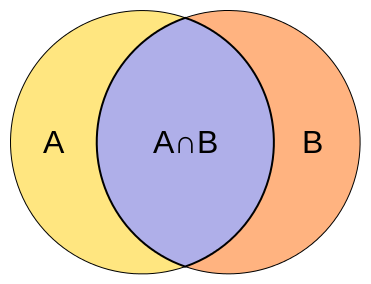
\includegraphics[width=0.20\textwidth]{images/Intersection_of_sets_A_and_B.png} 
    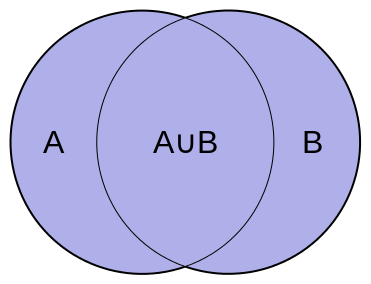
\includegraphics[width=0.20\textwidth]{images/Union_of_sets_A_and_B.png}
    \caption{Intersection and union of two sets $ A $ and $ B $ \cite{intersectionImage,unionImage}}
\end{figure}

Calculating the Jaccard coefficient for two sets and a total of $ n $ items has a complexity of $ O(n^2) $. For high dimensional sets, sets that contain a lot of items, which have therefor a large $ n $, the curse of dimensionality applies very quickly.\\